%% Преамбула TeX-файла

% 1. Стиль и язык
\documentclass[utf8x]{G7-32} % Стиль (по умолчанию будет 14pt)
\usepackage[T2A]{fontenc}
\usepackage[russian]{babel}
% Остальные стандартные настройки убраны в preamble.inc.tex.
\sloppy

% Настройки стиля ГОСТ 7-32
% Для начала определяем, хотим мы или нет, чтобы рисунки и таблицы нумеровались в пределах раздела, или нам нужна сквозная нумерация.
\EqInChapter % формулы будут нумероваться в пределах раздела
\TableInChapter % таблицы будут нумероваться в пределах раздела
\PicInChapter % рисунки будут нумероваться в пределах раздела

% Добавляем гипертекстовое оглавление в PDF
\usepackage[
bookmarks=true, colorlinks=true, unicode=true,
urlcolor=black,linkcolor=black, anchorcolor=black,
citecolor=black, menucolor=black, filecolor=black,
]{hyperref}

% Изменение начертания шрифта --- после чего выглядит таймсоподобно.
% apt-get install scalable-cyrfonts-tex

%\usepackage[numbers,sort&compress]{natbib}


\IfFileExists{cyrtimes.sty}
    {
        \usepackage{cyrtimespatched}
    }
    {
        % А если Times нету, то будет CM...
    }

\usepackage{graphicx}   % Пакет для включения рисунков

% С такими оно полями оно работает по-умолчанию:
% \RequirePackage[left=20mm,right=10mm,top=20mm,bottom=20mm,headsep=0pt]{geometry}
% Если вас тошнит от поля в 10мм --- увеличивайте до 20-ти, ну и про переплёт не забывайте:
\geometry{right=20mm}
\geometry{left=30mm}


% Пакет Tikz %%%/// МНЕ НЕ НУЖНО, это для черчения фигур
%\usepackage{tikz}
%\usetikzlibrary{arrows,positioning,shadows}

% Произвольная нумерация списков.
%\usepackage{enumerate} %%%/// МНЕ НЕ НУЖНО, это для custom наименований пунктов списка

% ячейки в несколько строчек
\usepackage{multirow}

% itemize внутри tabular
\usepackage{paralist,array}


% Настройки листингов.
% 8 Листинги

\usepackage{listings}

% Значения по умолчанию
\lstset{
  basicstyle= \footnotesize,
  breakatwhitespace=true,% разрыв строк только на whitespacce
  breaklines=true,       % переносить длинные строки
%   captionpos=b,          % подписи снизу -- вроде не надо
  inputencoding=koi8-r,
  numbers=left,          % нумерация слева
  numberstyle=\footnotesize,
  showspaces=false,      % показывать пробелы подчеркиваниями -- идиотизм 70-х годов
  showstringspaces=false,
  showtabs=false,        % и табы тоже
  stepnumber=1,
  tabsize=4,              % кому нужны табы по 8 символов?
  frame=single
}

% Стиль для псевдокода: строчки обычно короткие, поэтому размер шрифта побольше
\lstdefinestyle{pseudocode}{
  basicstyle=\small,
  keywordstyle=\color{black}\bfseries\underbar,
  language=Pseudocode,
  numberstyle=\footnotesize,
  commentstyle=\footnotesize\it
}

% Стиль для обычного кода: маленький шрифт
\lstdefinestyle{realcode}{
  basicstyle=\scriptsize,
  numberstyle=\footnotesize
}

% Стиль для коротких кусков обычного кода: средний шрифт
\lstdefinestyle{simplecode}{
  basicstyle=\footnotesize,
  numberstyle=\footnotesize
}

% Стиль для BNF
\lstdefinestyle{grammar}{
  basicstyle=\footnotesize,
  numberstyle=\footnotesize,
  stringstyle=\bfseries\ttfamily,
  language=BNF
}

% Определим свой язык для написания псевдокодов на основе Python
\lstdefinelanguage[]{Pseudocode}[]{Python}{
  morekeywords={each,empty,wait,do},% ключевые слова добавлять сюда
  morecomment=[s]{\{}{\}},% комменты {а-ля Pascal} смотрятся нагляднее
  literate=% а сюда добавлять операторы, которые хотите отображать как мат. символы
    {->}{\ensuremath{$\rightarrow$}~}2%
    {<-}{\ensuremath{$\leftarrow$}~}2%
    {:=}{\ensuremath{$\leftarrow$}~}2%
    {<--}{\ensuremath{$\Longleftarrow$}~}2%
}[keywords,comments]

% Свой язык для задания грамматик в BNF
\lstdefinelanguage[]{BNF}[]{}{
  morekeywords={},
  morecomment=[s]{@}{@},
  morestring=[b]",%
  literate=%
    {->}{\ensuremath{$\rightarrow$}~}2%
    {*}{\ensuremath{$^*$}~}2%
    {+}{\ensuremath{$^+$}~}2%
    {|}{\ensuremath{$|$}~}2%
}[keywords,comments,strings]

% Подписи к листингам на русском языке.
\renewcommand\lstlistingname{\cyr\CYRL\cyri\cyrs\cyrt\cyri\cyrn\cyrg}
\renewcommand\lstlistlistingname{\cyr\CYRL\cyri\cyrs\cyrt\cyri\cyrn\cyrg\cyri}


% Полезные макросы листингов.
% Любимые команды
\newcommand{\Code}[1]{\textbf{#1}}


\begin{document}

\frontmatter % выключает нумерацию ВСЕГО; здесь начинаются ненумерованные главы: реферат, введение, глоссарий, сокращения и прочее.

% Команды \breakingbeforechapters и \nonbreakingbeforechapters
% управляют разрывом страницы перед главами.
% По-умолчанию страница разрывается.

% \nobreakingbeforechapters
% \breakingbeforechapters

%% Также можно использовать \Referat, как в оригинале
\begin{abstract}
тра-тата

\end{abstract}

%%% Local Variables: 
%%% mode: latex
%%% TeX-master: "rpz"
%%% End: 


\tableofcontents

%$tex

\Introduction

Целью данной работы является миссиологический анализ миссионерских проповедей Нового Завета на предмет особенности проповеди, зависивших от религиозной принадлежности адресатов. Для достижения поставленной цели необходимо:

\begin{itemize}
\item провести анализ миссионерских проповедей в Новом Завете: выявить внешний контекст и повлиявшие на проповедь факторы, структуру проповеди, внутреннюю логику, основное смысловое содержание, непосредственную реакцию на проповедь и возможные причины для этой реакции;
\item выделить в ходе анализа особенности, связанные с принадлежностью адресатов к иудаизму или язычеству
\end{itemize}

В качестве основы для миссиологического анализа проповедей, используется следующее определение миссионерского служения: "главное дело миссионера в его служении – возвещение людям в историческом времени керигмы Церкви и призыв к Покаянию через осознания себя и мира сего в бедственном положении в силу противоречия между предчувствием своего высшего призвания в прекраснейшем мире и реальностью господства зла в нём и в себе" (\cite{@ogk.mag.}, с. 66).
В данной работе мы рассматриваем и анализируем как основное содержание проповеди керигму, свидетельство о призвании человека и падшести мира, логику призыва к Покаянию.


Несмотря на вариативность миссионерских ситуаций и проповедников в Новом Завете, можно говорить, что "Новозаветные тексты... формируют единство в своём провозвестии единого Евангелия" (\cite{@dodd.apostolic}, с. 74).
Существуют определённые элементы "первоначальной керигмы", которые дают нам возможность называть проповедь миссионерской, т.е. благовестием \footnote{Эти понятия близки вплоть до тавтологии, т.к. "евангелия", "благие вести" – один из видов керигмы в современном апостолам государственном мире имперского Рима (см. подробнее \cite{@via.kerigma}}.


В исследовании для нас также значимо значение керигмы, подчёркнутое \cite{@bultman.theology_1} (с. 307): керигма – это "личное обращение... оно ставит человека перед вопросом... требуя от него решения".
Керигма апостольской миссионерской проповеди ожидает отклика, как его ждал от слушателей Иисус в Своей проповеди, и потому всегда есть "призыв к послушанию" \cite{@via.kerigma}.
В синоптических Евангелиях этот призыв резюмирован "двумя словами: кайтесь, веруйте" \cite{@dunn.edinstvo}.
Поэтому для нас важно наличие этого призыва в проповеди, а также непосредственная реакция слушателей во время проповеди и после.


Актуальность работы для современной миссиологии связана с тем, что "современное миссионерское служение Церкви основывается на двухтысячелетнем опыте православного свидетельства святоотеческой традиции"\cite{@rpc.concepcia} (31, с. 15).
Опыт апостольской проповеди интересен для нас не только как исторический, но и как практический.
Современный опыт христианского свидетельства отличается контекстом, но керигма не изменилась.
Что же касается опыта её применения в различных условиях, для этого многообразие новозаветной проповеди при единстве Благовестия для нас особенно ценно.
Наконец, при отсутствии ветхозаветных иудеев или язычников эллинистического толка в наше время, мы сталкиваемся с фундаменталистскими и секулярными течениями в самом христианстве, а также людьми вовсе не знакомыми с Писанием и Преданием церкви и открыто исповедающими служение языческим ценностям.
То, как подобным слушателям возвещалось христианство в 1 веке, актуально и для современной практики христианской миссии.


За основной источник миссиологического исследования Новозаветной проповеди мы берём книгу Деяний апостолов.
В книге Деяний изложены события после рождения Церкви, когда уже прозвучал призыв Иисуса проповедовать (ср. Мф 28:19, Лк 24:46-49, Мк 16:15, Ин 15:27).
\cite{@brown.vvedenie_1} называет Деян 1:8 "божественным планом миссионерства (10.2.3).
В книге описано множество ситуаций миссионерской проповеди, но таких мест, где, хотя бы частично, присутствует её текст, всего 12.
Среди них – 8 проповедей к иудеям и боящимся Бога из (бывших) язычников, 4 – к язычникам, не знающим Бога.
Их анализу посвящена данная работа.


\mainmatter % это включает нумерацию глав и секций в документе ниже


\chapter{ Особенности миссионерской проповеди иудеям и богобоязненным}
\label{cha:judes}
%
% % В начале раздела  можно напомнить его цель
%
Среди иудеев были не только евреи, но и обратившиеся в иудаизм из других народов: прозелиты, богобоязненные (не обрезавшиеся, но соблюдавшие Закон). Потому мы рассматриваем в качестве миссии иудеям проповедь ап Филиппа эфиопскому евнуху и проповедь ап Петра сотнику Корнилию, "мужу праведному и боящемуся Бога" с домочадцами.

\subsubsection*{Проповедь ап Петра в день Пятидесятницы (Деян 2:14-2:47)}
%%внешний контекст
После сошествия Св Духа на апостолов, они "начали говорить иными языками" (2:4), что привлекло внимание окружающих.
Так как был большой праздник Шавуот, в Иерусалиме присутствовало множество народу, как местных, так и приезжих "Иудеев, благоговейных людей из всякого народа под небом".
Слух о странном событии, случившимся с апостолами, собрал толпу, "пришедших в смятение", "изумлявшихся" и "дивившихся", т.к. каждый слышал, что апостолы говорили на его наречье.
К этим разноплемённым, но исповедавшим одну ветхозаветную веру людям, вышел со словом проповеди апостол Пётр.

Браун называет эту проповедь "фундаментальной формулировкой благовестия" в Деян (\cite{@brown.vvedenie_1}, 10.2.2).
В ней формируется керигма апостольской проповеди, отличной от проповеди Иисуса христологическим содержанием и исповеданием Иисуса воскресшим, Господом, Мессией, Сыном Божьим. 

%%структура проповеди и внутр. логика
\begin{center}
	\begin{longtable}{ |c|c|p{0.70\textwidth}| } 
 \hline
 стих & смысл & содержание \\ 
 \hline\hline
 2:16-21 & напоминание & пророчества Иоиля о сошествии Духа \\ 
 2:22-24 & керигма & предведение Божье об Иисусе, убийство и воскресение \\ 
 2:25-28 & напоминание & пророчество царя Давида о воскресении \\
 2:29-31 & толкование & Давид говорил о Христе \\
 2:32 & керигма & "Этого Иисуса воскресил Бог, чему все мы свидетели" \\
 2:33 & керигма & Иисус излил Духа на апостолов \\
 2:34-35 & напоминание & Давид пророчествовал о Господе \\
 2:36 & керигма & обличение: дом Израилев распял Господа и Христа \\
 2:38 & призыв & покатесь, креститесь, примите дар Святого Духа \\
 2:39 & керигма & обещание Божье – для всех, в т.ч. "дальних" \\ 
 \hline
\end{longtable}
\end{center}


В ходе проповеди, люди начали задавать вопросы ("Что нам делать, мужи братья?" 2:37), и возможно, вопросы не прекратились после, так как и "иными многими словами" апостол "свидетельствовал и увещал их".
И многие ("около трёх тысяч") крестились и вошли в общение и учение апостолов.

%%керигма
Керигма проповеди ап Петра: 
\begin{itemize}
 \item исповедание Иисуса Христом, о котором "предвидел Бог" и говорили пророки
 \item Иисуса воскресил Бог
 \item Иисус принял Духа от Бога и ниспослал Его на апостолов
 \item Иисус был распят
 \item Благая Весть теперь – для всех
\end{itemize}

Каждое возвещение апостол сопровождает ссылкой на Ветхий Завет: о Мессии и воскресении пророчествовал пророк Давид, о сошествии Духа – пророк Иоиль, обещание для "дальних" напоминает Ис 57:19,
а обличение "дома Израилева" в распятии Христа созвучно пророческим обличениям.
Апостол цитирует писание пророков и истолковывает, как пророчества раскрываются в Иисусе Христе.
Кроме того, что это подкрепляет его речь авторитетом Писания, а в слушателях – пробуждает память об уже воспринятом откровении,
толкование ап Петра раскрывает ранее непонятные и смутные смыслы о преодолении "тления" и наступлении "того Дня".
Он толкует то, о чём никто не мог говорить уверенно, и при том возвещает, что происходит это сейчас, у всех на глазах.

%%св-во о ч-ке и мире
Свидетельство о мире и человеке принимает образ эсхатологического исполнения: как в "тот День" (Иоиль 3:18), люди примут дар Святого Духа и получит отпущение грехов.
%% призыв к Покаянию
Это предваряется условием: покаянием и крещением (погружением) "во имя Иисуса Христа".

\subsubsection*{Проповедь апп Петра и Иоанна по исцелению хромого у Храма (Деян 3:1-4:4)}
%%внешний контекст
Апостолы продолжали ходить в храм для молитвы и теперь также для проповеди.
На ступенях они повстречали калеку, который не мог быть в храме из-за телесного изъяна, но просил милостыню у ворот.
В ответ на просьбу о милостыне, ап Пётр исцелил его от хромоты, и тот вошёл в храм, "ходя и скача и хваля Бога".
Бывшие в храме люди "исполнились ужаса и изумления" и "сбежался к ним (апостолам и исцелённому) в трепете весь народ в притворе, называемом Соломоновым".
К этим благочестивым иудеям обратил проповедь ап Пётр.

%%структура проповеди и внутр. логика
\begin{center}
	\begin{longtable}{ |c|c|p{0.55\textwidth}| } 
		\hline
		 стих & смысл & содержание \\
		   \hline\hline
		   3:12 & обращение & это чудо – не собственной силой апостолов \\
		   3:13a & керигма & Бог прославил Иисуса, "Отрока Своего" \\
		     3:13b-15a & керигма & вы отреклись и убили Начальника жизни \\
		     3:15b & керигма & Бог воздвиг Иисуса из мёртвых \\
		     3:16 & свидетельство & вера во имя Иисуса исцелила хромого \\
		      3:17 & обращение & вы отреклись по неведению \\
		      3:18 & напоминание & пророки предрекли страдания Христа \\
		       3:19-20 & призыв & "покайтесь и обратитесь" \\
		       3:21 & керигма, напоминание & Иисус на небе "до времён восстановления всего" \\
		       3:22-23 & напоминание & Моисей обещал о воздвижении Пророка "из братьев ваших" \\
		       3:24 & напоминание & Самуил и другие пророки "возвестили эти дни" \\
		       3:25 & напоминание & "вы сыны пророков и завета" \\
		       3:26 & керигма & Бог воскресил Иисуса и послал Его к каждому из вас, чтобы "отвратить от злых дел ваших" \\
		\hline
	\end{longtable}
\end{center}

%%керигма
Керигма проповеди апостола Петра:
\begin{itemize}
	\item Бог прославил Иисуса
	\item Иисус – "отрок" Божий
	\item Иисус был убит
	\item Бог воздвиг Иисуса из мёртвых
	\item Иисус придёт во "времена восстановления всего"
	\item Иисус послан к каждому
\end{itemize}

Помимо возвещения, апостол свидетельствует о чуде исцеления хромого "верой во имя Иисуса", обращает несколько раз внимание слушателей на самих себя, "мужей израильских", "братьев", к которым обращён призыв "Бога отцов ваших", и вспоминает пророчество Моисея, Самуила и "других пророков" об "этих днях" чудес.

%%св-во о ч-ке и мире
Свидетельство о мире и человеке опять звучит в эсхатологическом ключе: дни, о которых сказано у пророков, наступили, и, следовательно, чудеса не для изумления, а для "покаяния и обращения" к Сыну Божьему, о Котором все пророчества.

%% призыв к Покаянию
Апостол не успевает завершить проповедь призывом, так как "пока они говорили к народу, приступили к ним... и наложили на них руки и отдали под стражу" (4:1-3)
Однако, в 3:19-20 уже прозвучал призыв к покаянию, в 3:23 апостол предупреждает не слушающегося "Пророка Того", а в 3:26 говорит, что "Отрок" Божий послан Богом, "чтобы каждого отвратить от злых дел ваших".
Многих свидетельство исцеления и слово проповеди привело в Церковь (3:4).  


\subsubsection*{Проповедь апп Петра и Иоанна перед первосвященниками (Деян 4:5-21; 5:27-33)}
%%внешний контекст
После того, как апостолы были схвачены, собрался синедрион для решения по их вопросу, и их стали доправшивать, "какой силой или каким именем вы это сделали?".
Апостол Пётр, "исполнившись Духа Святого", начал проповедь перед первосвященниками, старейшинами и книжниками Израиля.


Увидев, что апостолов не переубедить, их изгнали с угрозами.
На следующий день они были вновь схвачены учащими в храме, и были подвергнуты новому допросу.
Апостол Пётр продолжил проповедь.

%%структура проповеди и внутр. логика
\begin{center}
	\begin{longtable}{ |c|c|p{0.70\textwidth}| } 
		\hline
		стих & смысл & содержание \\
		\hline\hline
		4:8-9 & обращение & вы допрашивайте тех, кто спас человека \\
		4:10 & свидетельство & хромой исцелён именем Иисуса Христа \\
		4:10b & керигма & Бог воздвиг Иисуса из мёртвых \\
		4:11-12 & керигма & вне Иисуса нет спасения \\
		4:19 & свидетельство & апостолы не могут не слушать Бога и не говорить о том, "что видели и слышали" \\
		5:29 & свидетельство & смысловой повтор 4:19 \\
		5:30 & обращение & обличение: вы умертвили Иисуса \\
		5:30-31 & керигма & Бог воздвиг Иисуса из мёртвых \\
		5:31b & керигма & Иисус – Начальник и Спаситель, в Котором возможно покаяние и отпущение грехов Израиля \\
		5:32 & керигма & Бог дал Духа Святого "повинующимся Ему" \\
		\hline
	\end{longtable}
\end{center}

Апостол Пётр в каждое обращение к слушающим вкладывает обличение: это они распяли Иисуса, они нуждаются в покаянии.
То, что они "дети Авраама", а Бог – "Бог их отцов", только усугбляет ситуацию, так как они погубили Того, Кого избрал и воздвиг от смерти Бог.



%%керигма
Керигма проповеди апостола Петра:
\begin{itemize}
	\item Бог воздвиг Иисуса из мёртвых
	\item вне Иисуса нет спасения
	\item в Иисусе возможно покаяние и отпущение грехов
	\item Бог даёт Духа "повинующимся Ему"
\end{itemize}

%%св-во о ч-ке и мире
Свидетельство о человеке и мире раскрывается в Иисусе: человеку необходимо обрести спасение, которое есть только "в имени Иисуса".

%% призыв к Покаянию
В слове апостола нет прямого призыва к обращению, он завуалирован в параллели между словами обличения и возвещением покаяния и отпущения грехов в Иисусе, Спасителе.

По итогам проповеди, апостолы едва не были осуждены на смерть, но по ходатайству фарисея и уважаемого законоучителя Гамалиила, были отпущены после бичевания.


\subsubsection*{Проповедь Стефана (Деян 7:2-60)}
%%внешний контекст
Дьякон Стефан, "полный благодати и силы", стал известен благодаря чудесам и знамениям.
Когда члены синагоги либертинцев, киринейцев и александрийцев затеяли с ним спор, им не удалось взять верх, и были найдены лжесвидетели, оклеветавшие юношу.
Перед судом Синедриона, после обвинений в хуле на Закон и Моисея, Стефану было дано слово и он начал проповедовать.
Браун упоминает, что ни одна из речей апостолов в Деян не приводится столь тщательно разработанной (в рамках написания текста) как речь Стефана (\cite{@brown.vvedenie_1}, 10.2.2).
В ней настолько "нестандартное понимание Ветхого Завета", что она стала предметом споров о внешнем влиянии на иудейскую традицию (там же).

%%структура проповеди и внутр. логика
\begin{center}
	\begin{longtable}{ |c|c|p{0.55\textwidth}| } 
		\hline
		стих & смысл & содержание \\
		\hline\hline
		7:2-47 & напоминание, обращение & напоминание действия Бога в Священной истории от Авраама до Соломона \\
		7:37 & напоминание & пророчество Моисея о воздвижении "пророка из братьев ваших, как меня" \\
		7:39 & обращение & обличение: "<Моисею> не захотели покориться отцы ваши" \\
		7:48-50 & напоминание & Ис 66:1, нет рукотворного дома для Бога Вседержителя \\
		7:51-53 & обращение & обличение: "вы всегда Духу Святому противитесь, как отцы ваши" \\
		7:55-56 & керигма, свидетельство & небеса отверсты, Сын Человеческий стоит по правую сторону Бога \\
		7:59 & свидетельство & молитва: "Господи Иисусе, прими дух мой" \\
		7:60 & свидетельство & ходатайственная молитва за убивающих его \\
		\hline
	\end{longtable}
\end{center}

%%керигма
Керигма проповеди Стефана:
\begin{itemize}
	\item небеса отверсты (что также может быть свидетельством о собственном пророческом даре от Духа
	\item Сын Человеческий стоит по правую сторону Бога
\end{itemize}

В проповеди Стефан, как делал Сам Иисус, не говорит прямо о Нём, но ясно даёт Его образ в служении Моисея "который принял слова живые, чтобы дать вам".
Он обличает слушателей в отвержении Моисея "которому не захотели покоиться отцы ваши" и всего обетования Божьего, данного ещё Аврааму.
А уже в этой борьбе с пророками совершается отвержение "Праведного, Которого предателями и убийцами вы теперь сделались".

%%св-во о ч-ке и мире
Стефан свидетельствует как пророк, его слова об "отверстых небесах" имеет параллель в пророческом тексте: "отверзлись небеса, и я видел видения Божии" (Иез 1:1, Син.).
А параллель с Дан 7:13-14 ("с облаками небесными шёл как бы Сын Человеческий... и Ему дана власть, слава и царство... и Царство Его не разрушится") приводит к мысли о свершившимся обетовании Бога, наступлении конца времени и Царства Бога.
Стефан свидетельствует о человеке и мире, что наступило время последнего суда и последнего выбора человека быть с Богом или отвергнуть Его.
Небо уже открыто и ждать какого-то ещё исполнения пророчеств не следует.

%% призыв к Покаянию
В словах Стефана нет прямого призыва к Покаянию, подобного призывам в проповедях ап Петра.
Есть сочетание обличения, свидетельства об исполнении обетования Бога и личная ходатайственная молитва за своих слушателей и губителей, что можно назвать личным покаянием за их грехи.

Прямое следствие проповеди – мученическая смерть Стефана.
Но, существует мнение, что его свидетельство сыграло значительную роль в истории Савла.
Так, Браун пишет "как смерть Иисуса не была Его концом, поскольку апостолы обрели Его Дух... так и смерть Стефана не была его концом, ибо её видит юноша по имени Савл... ему суждено продолжить дело Стефана" (\cite{@brown.vvedenie_1}, 10.2.2).


\subsubsection*{Проповедь ап Филиппа эфиопскому евнуху (Деян 8:26-40)}
%%внешний контекст
Апостол Филипп по повелению ангела идёт по пустынной дороге "от Иерусалима к Газе", и встречает Эфиопа, евнуха, вельможу Эфиопской царицы.
Эфиоп читал пророка Исайю и был на поклонении в Иерусалиме, откуда возвращался.
По велению ангела, ап Филипп начинает с ним разговор, после которого он крестится во имя Иисуса.

%%структура проповеди и внутр. логика
\begin{center}
	\begin{longtable}{ |c|c|p{0.55\textwidth}| } 
		\hline
		стих & смысл & содержание \\
		\hline\hline
		8:31 & обращение & понимает ли Эфиоп, что читает из пророка Исайи \\
		8:35 & напоминание, керигма & "начав от этого писания, благовествовал ему Иисуса" \\
		8:37 & керигма & евнух может креститься, если верует от всего сердца \\
		\hline
	\end{longtable}
\end{center}

%%керигма
В тексте Деян не приведена проповедь ап Филиппа, поэтому мы не можем сказать точно о её керигматической части.
Как минимум, это слово об исполнении писаний и пророчеств в Иисусе, а также универсальность откровения Нового Завета: возможность и необходимость крещения в Иисуса для каждого верующего "от всего сердца", независимо от национальных или физиологических предпосылок (ср. с запретом во Втор 23:1).
В этой универсальности – и новое откровение о человеке и мире: наступило время исполнения пророчеств, и каждый может и должен обратиться сердцем к Богу и сделать конкретный шаг: креститься. \footnote{У пророков уже звучало это сочетание эсхатологического времени и возможности иноплеменника и евнуха войти в дом и храм Божий (ср. Ис 56:3-5)}


По итогу проповеди, евнух сам спрашивает о возможности креститься и принимает крещение от ап Филиппа.
После ухода Филиппа, он "продолжал, радуясь, свой путь".

\subsubsection*{Проповедь ап Петра сотнику Корнилию с домочадцами и друзьями (Деян 10:24-48)}
%%внешний контекст
Эта проповедь продолжает "изменение правил", заложенное в крещении евнуха: Божье слово обращено к людям не из народа Израиля.
Хотя речь идёт о людях, знающих Закон, а именно "благочестивом и боящимся Бога со всем домом своим... молящимся Богу постоянно" сотнике Корнилии, они по-прежнему имеют статус "внешних".
Это оказывается столь сильным препятствием, что и для сотника, и для ап Петра требуется прямое Божье откровение, чтобы сделать шаг навстречу друг другу.

Получив видение от Бога о снятии запрета на нечистую пищу, ап Пётр преодолевает свои сомнения и приходит вслед за вестниками от Корнилия в его дом.
Корнилий созвал "родственников своих и ближайших друзей", чтобы "послушать речей" апостола

%%структура проповеди и внутр. логика
\begin{center}
	\begin{longtable}{ |c|c|p{0.55\textwidth}| } 
		\hline
		стих & смысл & содержание \\
		\hline\hline
		10:26 & свидетельство & "сам я тоже человек" \\
		10:28-29 & свидетельство & Бог указал не называть человека нечистым, "потому я пришёл" \\
		10:34-35 & керигма & Бог обращается к каждому "боящемуся Его и делающему правду" \\
		10:36 & керигма & Иисус Христос – "Господь всех" \\
		10:37-38 & напоминание & проповедь Иоанна Крестителя, жизнь Иисуса из Назарета \\
		10:38 & керигма & Иисус исполнял пророчества "благотворя и исцеляя", "Бог был с Ним" \\
		10:39 & керигма & Иисус был убит на кресте \\
		10:40-41 & керигма & Бог воздвиг Иисуса из мёртвых \\
		10:39-42 & свидетельство & мы – свидетели Его проповеди и воскресения \\
		10:42 & керигма & Иисус – "поставленный Богом Судия живых и мёртвых" \\
		10:43 & керигма, напоминание & свидетельство пророков – о Нём; в Нём – отпущение грехов верующим \\
		10:47 & свидетельство & Дух Святой сошёл на язычников, а значит и в крещении им нельзя отказать \\
		10:48 & призыв & повеление креститься \\
		\hline
	\end{longtable}
\end{center}

%%керигма
Керигма проповеди ап Петра:
\begin{itemize}
	\item Божье откровение универсально и обращено к каждому "боящемуся Его и делающему правду"
	\item Иисус Христос – Господь
	\item в Иисусе исполнились пророчества
	\item Иисус был убит на кресте
	\item Бог воздвиг Иисуса из мёртвых
	\item Иисус – Судия живых и мёртвых
	\item в Иисусе – отпущение грехов и спасение человека
	\item теперь Дух Святой сходит на людей, даже не принадлежащих народу Израиля по крови
\end{itemize}

%%св-во о ч-ке и мире
Апостол Пётр приносит новое свидетельство о человеке, основанное на собственном, новом для себя откровении.
Человек не может быть назван "нечистым" и не может быть отвергнут Богом по какому-либо внешнему признаку.
Дух Святой ниспослан Богом для каждого верующего во имя Иисуса.
Помимо факта прихода к "язычникам" и свидетельства о сошествии на них Духа, ап Пётр говорит о себе "сам я тоже человек", никак не выделяя ни своего апостольства, ни принадлежности израильскому народу.

Ещё одно важное свидетельство – Иисус – "Судия живых и мёртвых", т.е. свидетельство о Суде, на который предстанет (или уже предстаёт) каждый человек.

%% призыв к Покаянию
Призыв апостола креститься звучит уже в ответ на сошествие Духа Святого на Корнилия с друзьями и домочадцами.

\subsubsection*{Проповедь ап Павла в Антиохии Писидийской (Деян 13:14-44)}
%%внешний контекст
Апостол Павел со спутниками по повелению Духа Святого, путешествовали и проповедовали в Иудейских синагогах.
В Писидийской Антиохии в синагоге их пригласили сказать "слово наставления к народу" после чтения Закона и Пророков, и ап Павел стал говорить.

%%структура проповеди и внутр. логика
\begin{center}
	\begin{longtable}{ |c|c|p{0.70\textwidth}| } 
		\hline
		стих & смысл & содержание \\
		\hline\hline
		13:16 & обращение & "мужи Израильские и боящиеся Бога, послушайте" \\
		13:17-22 & напоминание & рассказ о Священной истории от Египетского плена до царя Давида \\
		13:23 & керигма & к Израилю пришёл Иисус Спаситель, сын Давида \\
		13:24-25 & напоминание & свидетельство Иоанна Крестителя об Иисусе \\
		13:26 & обращение & "нам послано слово спасения этого" \\
		13:27-29 & керигма & Иисус был отвергнут "начальниками" и "живущими в Иерусалиме" и распят \\
		13:30 & керигма & Бог воздвиг Иисуса из мёртвых \\
		13:31 & свидетельство & мы и многие другие – свидетели Его воскресения \\
		13:32-37 & керигма & в Иисусе исполняются пророчества \\
		13:33-35 & напоминание & Пс 2:7, "милости, обещанные Давиду" (ср. Иез 37:24, Ос 3:5), Пс 88:49 \\
		13:38-39 & керигма & во Христе – отпущение грехов и Спасение, которого не может быть в Законе \\
		13:40-41 & призыв & покайтесь ("презрители, подивитесь и сгиньте") \\
		13:41 & керигма & наступил день, когда "дело делаю Я (Господь)" \\
		\hline
	\end{longtable}
\end{center}

%%керигма
Керигма апостола Павла:
\begin{itemize}
	\item пришёл Иисус, Спаситель
	\item Иисус – сын Давида
	\item в Иисусе сбываются пророчества
	\item наступили дни Господа, возвещённые в пророчествах
	\item Иисуса отвергли и распяли
	\item Бог воздвиг Иисуса из мёртвых
	\item в Иисусе Христе возможно прощение грехов, невозможное по Закону
\end{itemize}

%%св-во о ч-ке и мире
Апостол Павел свидетельствует, что человек может быть прощён и спасён, если примет Иисуса Христа.
Мир находится в решающей стадии: пророчества сбываются, Господь "дело делает" своё, и для каждого встаёт вопрос о покаянии.

%% призыв к Покаянию
Свой призыв апостол Павел произносит словами, "сказанными у Пророков": "Посмотрите, презрители, подивитесь и сгиньте, потому что дело делаю Я в дни ваши, дело, которому вы никак не поверите, если кто расскажет вам" (ср. Ис 5:24, 28:14-15)

По итогам проповеди, апостола со спутниками просили проповедовать в следующую субботу, а многие последовали за ними и начали научаться.
Слухи разошлись и в следующую субботу "почти весь город собрался слушать слово Божие".

\subsubsection*{Проповедь ап Павла перед обвинителями в Иерусалиме (Деян 22:1-24)}
%%внешний контекст
В Иерусалиме, в храме, Апостол Павел был обвинён, якобы он осквернил храм введением в него язычников.
Едва не растерзанный толпой, он был взят под стражу римским трибуном с воинами, но попросил о возможности принести перед обвинителями оправдательную речь.
Трибун дал такую возможность.

%%структура проповеди и внутр. логика
\begin{center}
	\begin{longtable}{ |c|c|p{0.70\textwidth}| } 
		\hline
		стих & смысл & содержание \\
		\hline\hline
		22:1 & обращение & – \\
		22:3-5 & свидетельство & жизнь ап Павла до обращения: наставленный в Законе и гонитель христиан \\ 
		22:6-21 & свидетельство & обращение, исцеление Павла и послушание от Бога идти к язычникам \\
		22:8 & керигма & Иисус Назорей – Господь \\
		22:16 & керигма & крестясь и "призвав имя Его" человек "смывает" грехи \\
		22:21 & керигма & Бог посылает на проповедь к язычникам \\
		\hline
	\end{longtable}
\end{center}

%%керигма
Апостол Павел говорит в своё оправдание и больше приносит личное свидетельство, прямо и честно рассказывает о себе, проводя параллели между собой и слушающими ("как все вы сегодня" Деян 22:3).
Но, так как собственную жизнь он строит на Божьем откровении, его свидетельство в себе косвенно заключает керигму (как бы к нему самому обращённую):
\begin{itemize}
	\item Иисус – Господь
	\item в Иисусе – Спасение и прощение грехов
	\item откровение Божье теперь и для язычников
\end{itemize} 

%%св-во о ч-ке и мире
Свидетельство о человеке прежде всего в универсализме Божьего Слова, теперь обращённого ко всем народам, а также в возможности прощения грехов в крещении и "призвании имени" Иисуса Христа.

%% призыв к Покаянию
Апостол Павел не успевает призвать слушающих к покаянию, но приносит собственное свидетельство покаяния, в т.ч. публично признавая, что "сочувствовал и стерёг одежды убивавших" Стефана.

\subsection*{Сравнительный анализ миссионерских проповедей иудеям и "богобоязненным"}

В проповеди иудеям значительную роль играет возвещение исполнения ветхозаветных пророчеств.
Как для самих апостолов, так и для их окружения, выросшего в среде, где Закон определял всю общественную жизнь, а Пророки возвещали основные духовные чаяния, свидетельство о Христе в этих текстах играло значительную роль.
Их отношение к тексту, при этом, было довольно свободным, в свете уже состоявшейся жизни, смерти и воскресения Христа.
Так, Данн прибегает к термину цитаты-"пешер", цитаты-толкования, возникавшей "когда сводили воедино данность текста и данность евангельской традиции" (\cite{@dunn.edinstvo} § 24).
Такие "новозаветные цитаты из Ветхого Завета суть интерпретации", а не "независимый авторитет" (там же).
Опираясь на это свидетельство и толкуя их в свете Евангелия, апостолы проповедуют исполнение обетованного Богом, исполнение пророчеств, продолжая проповедь Христа о "приблизившемся Царстве".


В 6 из 8 проповедей проповедник прямо ссылается на пророческие тексты, и говорит об их исполнении.
В Антиохии Писидийской ап Павел говорит о Христе как "сыне Давида" и ссылается на проповедь «современного» ему пророка Иоанна Крестителя, а перед толпой гонителей в Деян 22 самого себя, воспитанного в Законе "у ног Гамалиила", ставит свидетелем исполнения ветхозаветных обетований и надежд.
Эти толкования отличаются от толкований "книжников" и звучат "со властью", так как исповедуют как уже случившееся то, что в писаниях только ожидалось.


Стефан исповедует перед смертью, что "Небеса отверсты" и вспоминает видения апокалиптических глав пророка Даниила.
В Антиохии ап Павел говорит об исполнении "милостей, обещанных Давиду" (Деян 13:33) и о том, что ныне "Дело делаю Я (Господь)" (13:41).
В проповеди после сошествия Духа Святого, апостол Пётр толкует это явление словами пророка Иоиля (и, в свою очередь, толкует пророка этим исполнением у всех на глазах).
После исцеления хромого у ворот храма, апостол Пётр говорит, что нет нужды удивляться чудесам, так как наступило время чудес, которое возвещали Пророки.
Это удивительное единодушие апостольского толкования пророческих текстов подражает эсхатологичности проповеди Самого Иисуса.


Эсхатологическая весть для знавших Писание и живших в среде, полной апокалиптических настроений и проповедей (напр. проповедь Иоанна Крестителя), разворачивало людей к знакомым словам Писания, а слова – раскрывала по-новому для слушателей (подобно тому как делал Иисус, напр. в Лк 24:12-35).
Пророчество о Дне Господа, о наступлении Царства раскрывалось как уже сбывающееся.
Уже в проповеди Иоанна Крестителя зазвучала эта нота незамедлительности наступления Царства, и перед слушающим вставал вопрос: что в связи с этим нужно делать\footnote{Который они озвучивали прямо во время проповеди, судя по: Лк 3:10-14, Деян 2:37, 9:6, 16:30}?


На это у апостолов есть ответ, что также отличает их от иудейских апокалиптиков: "В то время как чаяния иудейской эсхатологии были неопределенными или выраженными чисто символическим языком, апокалиптическая надежда христианства сосредоточивалась на конкретном человеке" (\cite{@dunn.edinstvo}, § 69), Иисусе Христе.
Иисус исповедуется как Судья, Господь и Спаситель, а в Деян 3:13 – "отрок" Божий.
В Нём возвещается спасение Израиля и отпущение грехов, которые невозможно простить по Закону (Деян 13:38-39, 22:16).


Есть ещё один аспект проповеди иудеям со ссылкой на ветхозаветные писания.
Это обличение, что особенно раскрывается в толковании Стефаном священной истории как истории непослушания и отступничества, вплоть до нарушения воли Божьей строительством рукотворного храма.
У других проповедников обличение не столь радикально, но отговорка "отец у нас – Авраам" (Лк 3:8) обращена против иудеев.
Они не узнали Христа, прославленного Богом, Спасителя, и распяли его.
Потому все чаяния их веры теперь безнадёжны, если они не крестятся во имя Иисуса, ведь в Нём исполняется их обетование.


Наряду со смертью Иисуса, в 6 проповедях сказано о воскресении (в разговорах с Корнилием и евнухом Эфиопом этот эпизод не приведён).
Это – ещё одно прямое возвещение того, о чём в словах пророках только упомянается и что едва ли поддавалось внятному толкованию вне победы Иисуса Христа над смертью.


В эпизодах с "боящимися Бога" Эфиопом и Корнилием с домочадцами и друзьями есть так же возвещение универсальности Божьего призыва и крещения во имя Иисуса.
Вера – не для определённого народа или физической чистоты, но от чистоты сердца "боящихся Его (Бога) и делающих правду" (Деян 10:34-35).
Обретающие таким образом Христа как Господа получают прощение своих грехов и освобождение от них и дары Святого Духа (Деян 10:47).


%%% Local Variables:
%%% mode: latex
%%% TeX-master: "rpz"
%%% End:



%&tex
\chapter{Миссиологический анализ проповедей иудеям}
\label{cha:hellenes}

В этом разделе рассмотрены 4 проповеди: в Листрах, в Афинах, перед прокуратором Феликсом, а также перед царём Агриппой \footnote{Хотя Агриппа II и был по происхождению иудей, он рос в Риме при императорском дворце и был скорее римского воспитания, чем иудейского. Его сестра, Друзилла, упомянутая в Деян 24, открыто перешла в язычество и была замужем за прокуратором Феликсом.}.

\section{Миссиологический анализ проповедей иудеям}
\subsubsection*{Проповедь ап Павла в Листрах (Деян 14:8-18)}
% контекст
После гонений со стороны иконийских иудеев, ап Павел со спутниками бежал в Ликаонские города.
В городе Листра ап Павел исцелил хромого от рождения человека, что вызвало своеобразное религиозное пробуждение в местных жителях.
Решив, что перед ними – ходящие по земле боги, они собрались принести им жертву.
Остановив их, ап Павел и Варнава обратились к ним с проповедью.

%%структура проповеди и внутр. логика
\begin{center}
	\begin{tabular}{ |c|c|c| }
		\hline
		стих & смысл & содержание \\
		\hline\hline
		14:15a & обращение, свидетельство & апостолы – не боги, а люди, несущие благую весть \\
		14:15b & керигма & человек должен обратиться от "суетных богов" к Богу живому, Творцу \\
		14:16-17 & керигма & Бог живой свидетельствовал о Себе людям добром и радостью, оставляя людям свободу \\
		14:18 & призыв & не приносить жертвы "суетным богам" \\
		\hline
	\end{tabular}
\end{center}

%%керигма
Керигма в проповеди ап Павла и Варнавы:
\begin{itemize}
	\item человек должен отказаться от идолов ради служения одному Богу живому
	\item истинный Бог – Творец мира
	\item от Бога – всё доброе и радость в жизни всех людей
	\item Бог оставляет человеку свободу "ходить своими путями"
	\item Бог "свидетельствует о Себе" и призывает к Себе
\end{itemize}

%%св-во о ч-ке и мире
Мир был сотворён Богом, и всё доброе в мире – от Бога. 
Идолы – "суетные боги", которым не следует поклоняться.
Человек свободен выбирать свой путь.

%% призыв к Покаянию
В словах проповеди, изложенных в Деян 14:8-18 не звучит прямого призыва, но из приведённых слов и фразы "успокоили народ, чтобы не приносили им жертвы", можно заключить наличие призыва оставить идолопоклонство.

%%реакция на проповедь
Несмотря на клевету на апостола и Варнаву со стороны иудеев, в Листре и близлежащих городах появились ученики и общины, которые они после наставляли (Деян 21-23).

\subsubsection*{Проповедь ап Павла в Ареопаге (Деян 17:16-34)}

% контекст
Апостол Павел ожидал спутников в Афинах и "дух в нём возмущался, видя, что город полон идолов".
Помимо обычной проповеди в синагоге, он начал разговаривать "на полащди каждый день со случайными встречными".
Философы и другие, кто "ничем другим не заполняли свои досуги как тем, чтобы говорить или слушать что-нибудь новое", заинтересовались и попросили рассказать в Ареопаге об этом "новом учении".

%%структура проповеди и внутр. логика
\begin{center}
	\begin{tabular}{ |c|c|c| }
		\hline
		стих & смысл & содержание \\
		\hline\hline
		17:22 & обращение & "по всему вижу, что вы особенно богобоязненны" \\
		17:23 & напоминание & жертвенник "неведомому богу" \\
		17:24 & керигма & Бог Творец и Господь неба и земли не живёт в рукотворённых храмах \\
		17:25 & керигма & Бог – источник жизни \\
		17:26 & керигма & Бог сотворил людей и поставил "сроки и пределы их обитанию" \\
		17:27a & керигма & призвание человека – искать Бога \\
		17:27b & керигма & Бог "не далеко от каждого из нас" \\
		17:28a & керигма & Бог – источник бытия и движения \\
		17:28b & напоминание & "как и некоторые из ваших поэтов сказали: «Ведь мы Его и род»" \\
		17:29 & керигма & Бог не подобен идолу, сделанному человеком \\
		17:30 & керигма, призыв & Бог "теперь" возвещает людям, "всем и всюду", покаяние \\
		17:31a & керигма & будет день Суда вселенной "по праведности" \\
		17:32b & керигма & Суд – через "поставленного" Им Мужа, воскрешённого из мёртвых \\
		\hline
	\end{tabular}
\end{center}


%%керигма
Керигма проповеди ап Павла:
\begin{itemize}
	\item единый истинный Бог – Творец и Господь неба и земли
	\item Бог – начало всего: жизни, бытия, движения
	\item Бог не подобен идолам и созданиям человеческой мысли и не нуждается в рукотворённых храмах
	\item человек сотворён Богом и призван Его искать
	\item Бог "не далеко" от каждого человека
	\item Бог лично призывает каждого человека покаяться
	\item грядёт Суд над вселенной "по праведности"
	\item Бог избрал Мужа, Который будет судить и Которого воскресил из мёртвых
\end{itemize}

%%св-во о ч-ке и мире
Апостол свидетельствует о сотворённости и конечности мира, а также о том, что Суд над миром будет "по праведности".
Человек сотворён Богом, Бог всегда рядом, человек призван Его найти и прийти к Нему, ответив на Его призыв покаянием.
В "Муже, Которого Он поставил" побеждена смерть.

%% призыв к Покаянию
Апостол объявляет, что Бог лично изменил ход истории: времена неведения прошли, и Бог теперь возвещает "всем и всюду" необходимость покаяния.
Покаяние нужно, так как Суд над миром – "по праведности".

%%реакция на проповедь
Слова о воскресении мёртвых вызывают непонимание и многие начинают насмехаться, хотя кое-кто просит послушать об этом ещё раз.
Некоторые из слушавших уверовали (Деян 17:34).

\subsubsection*{Проповедь ап Павла прокуратору Феликсу (Деян 24:10-26)}
% контекст
Обвиняемый первосвященником Ананией и другими старейшинами в осквернении храма, ап Павел предстал перед судом прокуратора Феликса.
Когда апостолу позволили говорить в свою защиту, он произнёс проповедь.

%%структура проповеди и внутр. логика
\begin{center}
	\begin{tabular}{ |c|c|c| }
		\hline
		стих & смысл & содержание \\
		\hline\hline
		24:10 & обращение & – \\
		24:11-13 & апология & Павел не совершил ничего дурного \\
		24:14-15 & свидетельство & "служу Богу отцов наших... надежду имея на Бога" \\ 
		24:14 & керигма & есть Путь служения Богу, согласно с Законом и Пророками \\
		24:15 & керигма & будет воскресение праведных и неправедных \\
		24:16 & свидетельство & потому апостол старается жить в непорочной совести \\
		24:17-20 & апология & Павел не совершил ничего дурного \\
		24:21 & свидетельство & ап Павел верует в воскресение мёртвых и готов на том стоять \\
		24:25 & призыв & призыв к "праведности" и "обладанию собой", т.к. будет Суд \\
		\hline
	\end{tabular}
\end{center}

%%керигма
Керигма в проповеди ап Павла:
\begin{itemize}
	\item существует Путь служения Богу
	\item грядёт воскресение праведных и неправедных
	\item требуется жить в "непорочной совести пред Богом и людьми", праведно, обладая собой
\end{itemize}


%%св-во о ч-ке и мире
Апостол свидетельствует, что всякого человека ожидает воскресение, и от всякого требуется праведность и чистота совести.
Что же касается воскресения Христа, то до личной встречи с Феликсом и Друзиллой (24:24-26), апостол не говорит об этом.
Возможно, причина в том, чтобы проповедь изабвления от смерти не оказалась "смазана" оттенком внутренних распрей иудеев о неких спорных духовных авторитетах.

%% призыв к Покаянию
После 24:21 Феликс, "имея более точные сведения о Пути", отослал первосвященника и обвинителей и поместил ап Павла под стражу, чтобы через несколько дней прийти к нему с женой Друзиллой, Иудеянкой и "слушать его о вере во Христа Иисуса".
Тогда ап Павел продолжил проповедь призывом к покаянию и праведной жизни.
Из Деян 24:26 следует, что безуспешно, так как прокуратор Феликс испугался слов о будущем суде и "надеялся, что Павел даст ему денег".


\subsubsection*{Проповедь ап Павла перед царём Агриппой (Деян 26:1-31)}
% контекст
Не желая, чтобы его отдали в руки иудеев, способных убить его, ап Павел потребовал суда Кесаря (императора), что позволялось римскому гражданину под угрозой смертного приговора.
По приезду царя Агриппы, апостолу было позволено держать защитительную речь перед ним, "трибунами и виднейшими в городе людьми", и он произнёс проповедь. 

%%структура проповеди и внутр. логика
\begin{center}
	\begin{tabular}{ |c|c|c| }
		\hline
		стих & смысл & содержание \\
		\hline\hline
		26:2-3 & обращение & царь Агриппа назван "знатоком всех обычаев и спорных мнений Иудеев" \\
		26:4-22 & свидетельство & история воспитания, обращения, исцеления и служения апостола \\
		26:6-8 & напоминание & Иудеи, "усердно служа Богу", надеются на обещание от Бога \\
		26:15 & керигма & Иисус – Господь \\
		26:17 & керигма & Иисус имеет слово для язычников \\
		26:18 & керигма, призыв & необходимо обратиться "от тьмы к свету и от власти сатаны к Богу" \\
		26:18b & керигма & отпущение грехов возможно в вере в Иисуса \\
		26:20 & призыв & апостол возвещал язычникам каяться и творить "достойные покаяния" дела \\
		26:23 & керигма & Христос пострадал, но воскрес из мёртвых \\
		26:23b & керигма & проповедь Христа – для всех народов \\
		26:25 & апология & проповедь апостола – "слова истины и здравого смысла" \\
		26:26 & призыв & если Агриппа верит Пророкам, ему надо поверить в проповедь ап Павла \\
		26:29 & свидетельство & апостол надеется, что все уверуют во Христа \\
		\hline
	\end{tabular}
\end{center}

%%керигма
Керигма в проповеди ап Павла:
\begin{itemize}
	\item Иисус – Господь
	\item проповедь Христа – для всех народов
	\item во Христе возможно отпущение грехов
	\item Христос пострадал, но воскрес из мёртвых
	\item необходимо освобождение от власти сатаны и обращение к Богу, покаяние и творение "достойных покаяния дел"
\end{itemize}

%%св-во о ч-ке и мире
Апостол свидетельствует, что человек призван к свободе от власти греха и сатаны.
Проповедь Христа возвещает всем людям освобождение и отпущение грехов в вере в Него.
Обетование и надежда Иудеев – на воскресение, и это сбывается во Христе.

%% призыв к Покаянию
Апостол прямо обращается к царю Агриппе с призывом откликнуться на его проповедь, если он верит словам Пророков.
Как надлежит откликнуться – он говорит ранее, рассказывая о язычниках, которые покаялись и теперь творят "достояные покаяния дела".

%%реакция на проповедь
Неизвестно, какими были плоды проповеди кроме того, что Агриппа и его приближённые нашли, "что ничего достойного смерти или уз человек этот не делает".


\section{Особенности миссионерской проповеди язычникам в Новом Завете}
Основной особенностью проповеди язычникам стала необходимость проповедовать Единого Бога Творца и призывать к отказу от идолопоклонства.
В двух проповедях (Листры и Афины) присутствует это свидетельство, разное по форме, но единое в содержании.
Во всех случаях Бог исповедуется как:  
\begin{itemize}
	\item Творец и начало всего
	\item единый Бог для всех, а не для какого-либо народа
	\item Живой Бог, лично принимающий участие в жизни человека, с Которым возможны личные отношения
	\item истинный, отличающийся от созданий человеческих рук и мыслей (идолов)
	\item имеющий благое попечение о человеке и человечестве
\end{itemize}

В разговоре с простыми людьми (судя по всему, Листра – небольшой город), апостол ссылается не на философов и поэтов, а на действие Божье в жизни его слушателей: "подавая вам с неба дожди и времена плодоносные, исполняя пищею и радостью сердца ваши". 
Бог как пища, радость, дождь – един для всех и для каждого, близок и благ к каждому.
Кроме того, Он "позволил всем народам ходить своими путями", а значит лично принимает свободу человека и ждёт таких же личных отношений от него.


В Листрах Бог возвещается как создатель "неба и земли, и моря и всего, что в них", – как практически детским перечислением (ср. Пс 103) творения исповедуется Бог, как начало всего.
Совсем по-другому – в Ареопаге: "Сам дарует всем жизнь и дыхание и всё" (начало жизни), "произвёл род человеческий... предуставив сроки и пределы их обитанию", "«Ведь мы Его и род»" (начало людей), "в Нём мы живём и движемся и существуем" (начало бытия и движения).
Бог – конечный ответ на поиск "начал" в философии и личности человека (Отец, хотя бы как основатель рода человеческого).
И во всём – с акцентом на личностности Бога: "Бог не далеко от каждого из нас", "произвёл... род человеческий... искать Бога", – т.е., так же оставил свободу выбора пути, хоть и с личной заинтересованностью в близости.


Таким образом, в откровении о Едином Боге говорится и откровение о человеке как свободном, но призванном к духовному пути близости к своему Творцу.
Но человек ещё только призван стать таким, обратиться "от тьмы к свету и от власти сатаны к Богу" (Деян 26:18), получить отпущение грехов.
Как и в Лк, в Деян Царство Божье проповедуется как избавление человека от власти духов мира сего, от власти болезней и немощей и, в итоге, смерти (чему соответствует проповедь воскресения Христова как исполнения обетованного Пророками).


Эта свобода актуализируется в оставлении служения "руками человеческими" созданиям "печати искусства и мысли человеческой" в "рукотворённых храмах".
В проповедях перед Ареопагом, перед прокуратором Феликсом и перед царём Агриппой апостол наряду с возвещением свободы говорит о суде и покаянии, которые отличаются от привычных методов оценки человеческой жизни божественными силами (либо равнодушными, либо смотрящими на богатство приносимых даров).
Суд над вселенной будет "по праведности" (Деян 17:31), язычники, которым проповедовал ап Павел "обращались к Богу, творя дела, достойные покаяния" (Деян 26:18), и с прокуратором Феликсом апостол начинает говорить о необходимости изменения жизни: "обладании собой", "праведности" (Деян 24:24-25).
В Листрах же ап Павел и Варнава буквально силой останавливают языческую церемонию, которой хотели отметить местные жители чудо исцеления хромого.
Бог проповедуется как имеющий всё и, соответственно, не "имеющий в чём-либо нужду" от человека, но призывающий человека к себе через покаяние (обращение) (Деян 17:30).


Этот призыв, как исповедует апостол, теперь обращён ко "всем и всюду", потому что проходят "времена неведения", и определён день суда (Деян 17:30-31). 
Эсхатологический элемент керигмы, пробуждающий актуальную память знавшего слова пророков, для язычников был приниципиально новым свидетельством о мире, времени, истории\footnote{См. напр. \cite{@dunn.vvedenie}: "Апокалиптическая эсхатология принимает еврейское видение истории (практически уникальное для античности): история мыслится линейно... как движение вперёд к определённому концу и цели" (§ 66.3)}.
Без этого элемента возвещения Суда и призыв к покаянию как возможности для Спасения, были бы невозможны.


Интересно, что проповедуя в Ареопаге, апостол Павел отталкивается от архаического (вероятно, даже в то время) образа-мифа "неведомого бога", а не от представления о мире одной из популярных в то время философских школ.
Судя по цитатам, он был знаком с культурой и взглядами на устройство мира эллинистического мира.
Но, обращается к глубоко религиозному чувству трепета перед неведомым, тем отметая возможность расценить его речь как приглашение к философскому дискурсу.
Эта проповедь "не в убедительных словах человеческой мудрости" (1Кор 2:4) вызывает непонимание одних ("одни насмехались"), но интерес других ("мы послушаем тебя об этом ещё раз").


В рамках того же религиозного трепета перед неведомым, ап Павел в проповеди язычникам аппелирует к столь же неразрешимым загадкам сил природы и смерти.
Если по первому вопросу в иудейском мире ещё существовал ответ: надо поклоняться не силам, а Богу, от Которого всё произошло, то последний ставил в тупик и иудеев, и эллинов.
Его разрешение было возможно только в керигме Господа над всем, включая смерть, от которой Его избавляет Бог.


Апостол проповедовал то, что, вероятно, когда-то "пронзило" его самого, ведь "для самого апостола Павла важнейшим эсхатологическим событием, в котором живой Бог открыл... Свой замысел о спасении мироздания, стало \textit{воскресение Иисуса из мёртвых}"\cite{@wright.4to}.
Победа над смертью означала победу над грехом, а значит – полное освобождение от власти сатаны, полный и окончательный переход под власть Бога.
Отсюда – постоянство керигмы о воскресении Христа, несмотря на неготовность слушателей эллинистического воспитания.


%%% Local Variables:
%%% mode: latex
%%% TeX-master: "rpz"
%%% End:



\backmatter %% Здесь заканчивается нумерованная часть документа и начинаются ссылки и
            %% заключение

%$tex

\Conclusion % заключение к отчёту

В ходе анализа 12 миссионерских проповедий книги Деяний, были выделены структура, основное керигматическое содержание, логика призыва к Покаянию, свидетельство о человеке и мире в свете Новозаветного откровения.
Также, удалось выявить особенности проповеди для слушателей, живущих в иудейском Законе и знающих Бога Живого и для язычников.


Общей для всех случаев керигмой стало возвещение Христа, убитого и воскресшего, Господа и Судии, в Котором – освобождение от грехов.
Особенность проповеди Христа сказывается в том, что иудеям Его смерть и воскресение возвещаются как обличение, делающее недопустимым надежду на спасение в Законе и Пророках: народ Израиля не узнал и отверг Мессию и Спасителя.
Язычникам же Христос не всегда и не сразу возвещается прямо, не произносится и Его имя и происхождение, вероятно, чтобы не затушевать универсализм спасительной вести национальным оттенком.


Второе общее для всех случаев возвещение – близость Царства Божьего.
Все миссионерские проповеди Нового Завета носят эсхатологический оттенок исполнения пророчеств, наступления долгожданного Дня Господня, близости суда Христа, приходящего в силе.
И для иудеев, и для язычников, такая проповедь ставит вопрос радикально: прямо сейчас (или уже никогда) следует принять решение вверить себя Христу.
Основные формы такого возвещещения: интерпритационная проповедь Пророков как исполняющейся на глазах слушателей реальности, возвещение грядущего Суда, сам жанр керигмы-евангелия\footnote{Будучи формулой возвещения императорской власти, керигма в римском юридическом понимании не предполагала иной возможности кроме подчинения. Подробнее см. \cite{@via.kerigma}}.
Такое возвещение было испытанием и для самого проповедника, жизнь которого должна была соответствовать вести о приблизившемся Царстве.
Может быть, одна из причин, по которой эсхатологизм в современной миссионерской проповеди (в отличии от апокалиптизма, подробнее см. \cite{@dunn.vvedenie § 69} редок, и проповедь может не иметь той "соли" апостольской.


Эсхатологичность и проповедь Христа как Господа и Спасителя логически приводят к вопросу о дальнейших шагах.
Большинство проанализированных проповедей заканчивались призывом к покаянию и крещению.
И покаяние, и крещение проповедовались как дело открытого Богу сердца и чистой совести.
Потому оно было возможно для евнуха или необрезанных из язычников, и оставалось необходимым для "сынов Авраама", исполняющих Закон.


Основное различие между проповедью иудеям и язычником связано с необходимостью проповеди для последних Единого Живого Бога Творца и отречению от идолов ради Него.
Апостолы нигде не пропускали этого этапа проповеди и явно чувствовали разницу в проповеди язычникам.
Известные миссионеры ХХ века, такие как К. С. Льюис или митр. Антоний (Блум) хорошо чувствовали необходимость проповеди Живого Бога Отца миру, незнакомому с Ним, и находили слова для этого, понятные современному им человеку.
Первыми эту традицию проповеди среди язычников заложили апостолы, вышедшие с Благой Вестью за пределы Израиля.


Для любого современного миссионера, открывающего книгу Деяний, встанет вопрос о том, как обрести силу духа и слова апостолов.
Анализ проповедей показывает нам, как эти люди в разных ситуациях, перед разъярённой толпой или перед сельскими жителями поражёнными чудесами, перед собравшимися на досуг афинянами или на суде, подбирали слова, способные донести до слушателя ту керигму, которой жили сами.
Их собственное соответствие их возвещению позволило слову достигать сердца людей, и из их проповеди родилась христианская церковь.

%%% Local Variables: 
%%% mode: latex
%%% TeX-master: "rpz"
%%% End: 



% % Список литературы при помощи BibTeX
% Юзать так:
%
% pdflatex rpz
% bibtex rpz
% pdflatex rpz

\bibliographystyle{gost780u}
\bibliography{aspiro_1.0}

%%% Local Variables: 
%%% mode: latex
%%% TeX-master: "rpz"
%%% End: 


\appendix   % Тут идут приложения

\chapter{Источники XIV–XVвв. о введении женщин в алтарь на постриге или облачении}
\label{cha:appendix1}

\begin{figure}[h]
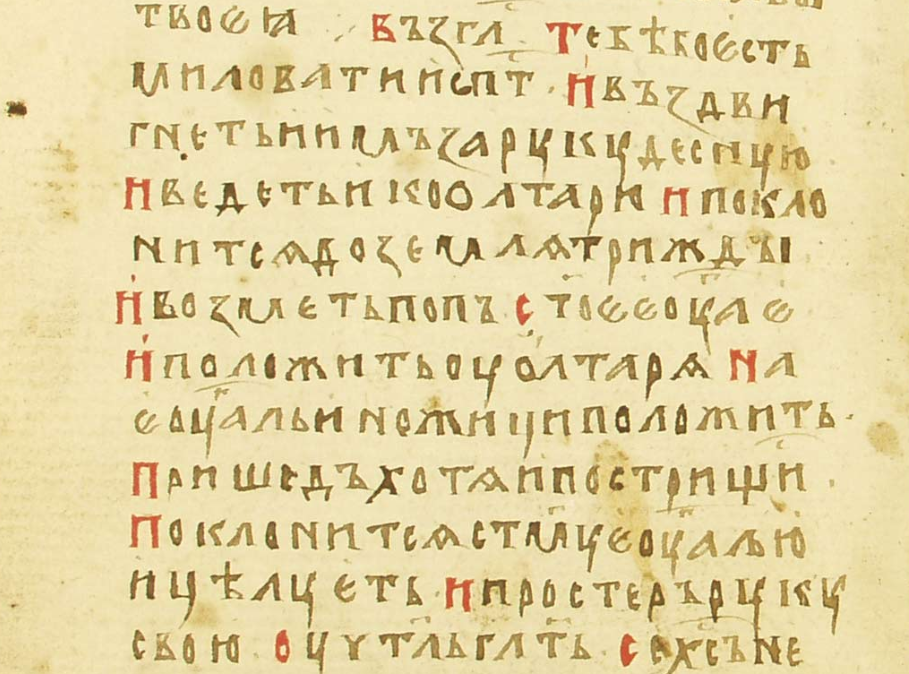
\includegraphics[width=1\linewidth]{14c._altar_hair}
\caption{Введение в алтарь на постриг. Требник XIVв. №998}
\label{14c._altar_hair}
\end{figure}

%%% Local Variables: 
%%% mode: latex
%%% TeX-master: "rpz"
%%% End: 

\chapter{Проповеди язычникам}
\label{cha:appendix2}

\subsection*{Проповедь ап Павла в Листрах (Деян 14:8-18}
8 И некий муж в Листрах, не владевший ногами, сидел; хромой от чрева матери своей, он никогда не ходил.

9 Он слышал, как говорил Павел, который, устремив на него взор и увидев, что он имеет веру, чтобы быть спасенным,

10 сказал громким голосом: встань на ноги твои прямо. И он вскочил и стал ходить.

11 Народ же, увидев, что сделал Павел, возвысил свой голос, говоря по-ликаонски: боги в образе человеческом сошли к нам.

12 И называли они Варнаву Зевсом, а Павла Гермесом, так как он держал речь.

13 И жрец Зевса, стоящего перед городом, доставив к воротам быков и венки, хотел с народом принести жертву.

14 Но апостолы Варнава и Павел, услышав, разорвали одежды свои и с криком бросились в толпу,

15 говоря: мужи, что это вы делаете? И мы – подобные вам люди, благовествующие вам, чтобы вы от этих суетных богов обратились к Богу живому, Который сотворил небо и землю, и море и всё, что в них,

16 Который в прошедших поколениях позволил всем народам ходить своими путями,

17 хотя и не переставал свидетельствовать о Себе, творя добро, подавая вам с неба дожди и времена плодоносные, исполняя пищею и радостью сердца ваши.

18 И говоря это, они едва успокоили народ, чтобы не приносили им жертвы.

\subsection*{Проповедь ап Павла в Ареопаге (Деян 17:16-34)}
16 И пока Павел ожидал их в Афинах, дух его в нем возмущался, видя, что город полон идолов.

17 Итак, он рассуждал в синагоге с Иудеями и чтущими Бога, и на площади каждый день со случайными встречными.

18 А кое-кто и из эпикурейских и стоических философов встречался с ним, и некоторые говорили: что хочет сказать этот пустослов? А другие: кажется, это проповедник чужих богов (потому что он благовествовал Иисуса и воскресение).

19 И взяв его, привели в Ареопаг и говорили: можем ли мы узнать, что это за новое учение, проповедуемое тобой?

20 Ибо странное что-то вкладываешь ты в наши уши. Вот мы и хотим узнать, что это может быть?

21 Афиняне же все и живущие у них чужестранцы ничем другим не заполняли свои досуги, как тем, чтобы говорить или слушать что-нибудь новое.

22 И Павел, став посредине Ареопага, сказал: мужи Афиняне, по всему вижу, что вы особенно богобоязненны.

23 Ибо, проходя и осматривая ваши святыни, я нашел и жертвенник, на котором было написано: "неведомому богу". Итак, что вы, не зная, чтите, я возвещаю это вам.

24 Бог, сотворивший мир и всё, что в нём, Он, Господь неба и земли, не в рукотворенных храмах обитает,

25 и не руками человеческими воздается Ему служение, как имеющему в чем-либо нужду: Он Сам дарует всем жизнь и дыхание и всё.

26 И произвёл Он от одного весь род человеческий: обитать по всему лицу земли, предуставив сроки и пределы их обитанию;

27 искать Бога, не коснутся ли они Его и не найдут ли, хотя и не далеко Он от каждого из нас.

28 Ибо в Нем мы живем и движемся и существуем, как и некоторые из ваших поэтов сказали: "Ведь мы Его и род".

29 Итак, будучи родом Божиим, мы не должны думать, что Божество подобно золоту, или серебру, или камню, носящим печать искусства и мысли человеческой,

30 Поэтому, оставив без внимания времена неведения, Бог теперь возвещает людям, всем и всюду, чтобы они каялись,

31 ибо Он определил день, когда будет судить вселенную по праведности, чрез Мужа, Которого Он поставил, дав удостоверение всем, воскресив Его из мертвых.

32 Услышав же о воскресении мертвых, одни насмехались, другие сказали: мы послушаем тебя об этом еще раз.

33 Так Павел вышел из среды их.

34 Но некоторые люди, примкнув к нему, уверовали: между ними и Дионисий Ареопагит и женщина, по имени Дамарь, и другие с ними.

\subsection*{Проповедь ап Павла прокуратору Феликсу (Деян 24:10-26)}
10 И ответил Павел, когда правитель сделал ему знак говорить: зная, что ты с давних лет судишь этот народ, я с легким сердцем буду защищать мое дело,

11 так как ты можешь узнать, что – не более двенадцати дней, как я пришел для поклонения в Иерусалим.

12 И не нашли меня ни в храме с кем-либо спорящим или вызывающим волнение народа, ни в синагогах, ни в городе,

13 и не могут доказать тебе того, в чем теперь обвиняют меня.

14 Но в том я признаюсь тебе, что на Пути, который они называют ересью, я, действительно, служу Богу отцов наших, веруя всему, что согласно с Законом и что написано у Пророков,

15 надежду имея на Бога, которую и сами они разделяют, – что будет воскресение и праведных и неправедных.

16 Потому я и сам стараюсь всегда иметь непорочную совесть пред Богом и людьми.

17 Через несколько лет я прибыл с целью передать милостыни народу моему и приношения.

18 При этом нашли меня очистившимся в храме, не с толпой и не с шумом,

19 нашли же какие-то Иудеи из Асии, которым надлежало бы быть здесь у тебя и обвинять, если бы у них было что против меня.

20 Или пусть они сами скажут, какое нашли они преступление, когда я предстал пред синедрионом,

21 кроме одного этого слова, которое я возгласил, стоя между ними: "за воскресение мертвых вы меня судите сегодня".

22 Но Феликс, имея более точные сведения о Пути, отослал их для дополнительного расследования, сказав: когда придет трибун Лисий, я рассмотрю ваше дело;

23 и дал распоряжение сотнику держать его под стражей, но давать ему некоторые послабления, и не препятствовать никому из близких его служить ему.

24 Несколько дней спустя, Феликс, прибыв с Друзиллой, женой своей, Иудеянкой, послал за Павлом и слушал его о вере во Христа Иисуса.

25 Но так как он говорил о праведности и обладании собой и о будущем суде, то Феликс, придя в страх, ответил: пока иди, а при случае я тебя вызову к себе.

26 В то же время он и надеялся, что Павел даст ему денег. Потому-то, часто за ним посылая, он и беседовал с ним.

\subsection*{Проповедь ап Павла перед царём Агриппой (Деян 26:1-31)}
1 И сказал Агриппа Павлу: тебе разрешается говорить за себя. Тогда Павел, протянув руку, начал свою защитительную речь:

2 во всём, в чем обвиняют меня Иудеи, царь Агриппа, я почитаю себя счастливым защищаться сегодня перед тобой,

3 потому особенно, что ты знаток всех обычаев и спорных мнений Иудеев. Поэтому прошу выслушать меня с долготерпением.

4 Жизнь мою от юности, протекавшую с самого начала среди народа моего в Иерусалиме, ведают все Иудеи,

5 зная обо мне издавна, если есть у них желание свидетельствовать – что жил я фарисеем, по строжайшему направлению в нашей вере.

6 И теперь я стою перед судом за надежду на обещание, бывшее от Бога отцам нашим,

7 исполнения которого надеются достичь наши двенадцать колен, усердно служа Богу день и ночь. За эту надежду, царь, и обвиняют меня Иудеи.

8 Почему у вас считается невероятным, что Бог воздвигает мертвых?

9 Ведь я и сам думал, что против имени Иисуса Назорея надо мне многое сделать.

10 Это я и делал в Иерусалиме, и многих из святых я заключил в тюрьмы, получив власть от первосвященников, и когда их убивали, подавал свой голос против них;

11 и по всем синагогам, многократно наказывая их, принуждал к хуле и, в чрезмерной против них ярости, преследовал их даже и в чужих городах.

12 В этих условиях, отправляясь в Дамаск с полномочиями и поручением от первосвященников,

13 я в полдень на дороге увидел, царь, свет с неба, сильнее солнечного блеска, осиявший меня и шедших со мной.

14 И когда все мы упали на землю, я услышал голос, говорящий мне на еврейском языке: "Саул, Саул, что ты меня гонишь? Трудно тебе идти против рожна".

15 Я сказал: "Кто Ты, Господи?" Господь сказал: "Я Иисус, Которого ты гонишь.

16 Но встань и стань на ноги твои, ибо Я для того явился тебе, чтобы поставить тебя служителем и свидетелем Моим, как ты Меня видел, и как Я явлюсь тебе,

17 избавляя тебя от народа и от язычников, к которым Я посылаю тебя,

18 открыть им глаза, чтобы обратились они от тьмы к свету и от власти сатаны к Богу, и чтобы получили они отпущение грехов и удел вместе с освященными, по вере в Меня".

19 Поэтому, царь Агриппа, я не оказал непослушания небесному видению,

20 но сперва находящимся в Дамаске и Иерусалиме, и по всей стране Иудейской, и язычникам возвещал, чтобы они каялись и обращались к Богу, творя дела, достойные покаяния.

21 За это Иудеи, задержав меня в храме, пытались расправиться со мной.

22 Итак, с помощью, которая приходит от Бога, я устоял до сего дня, свидетельствуя малому и великому, не говоря ничего, кроме того, о чем Пророки сказали и Моисей, что должно тому быть:

23 Христу – пострадать и, воскресши первым из мертвых, свет возвещать народу и язычникам.

24 Когда он так защищался, Фест громким голосом говорит: ты безумствуешь, Павел! Большая ученость доводит тебя до безумия.

25 А Павел говорит: я не безумствую, превосходнейший Фест, но возглашаю слова истины и здравого смысла.

26 Ибо знает об этом царь, которому я и говорю с дерзновением. Ведь я не верю, чтобы сокрыто было от него что-либо из этого; ибо не в углу это было совершено.

27 Веришь ли, царь Агриппа, Пророкам? Знаю, что веришь.

28 Но Агриппа Павлу: еще немного, и ты будешь убеждать меня сделаться христианином.

29 А Павел: молил бы я Бога, чтобы мало ли, много ли, не только ты, но и все слушающие меня сегодня, сделались такими же как и я, кроме этих уз.

30 И встал царь и правитель и Вереника и сидевшие с ними,

31 и удалившись, говорили между собой, что ничего достойного смерти или уз человек этот не делает.

%%% Local Variables: 
%%% mode: latex
%%% TeX-master: "rpz"
%%% End: 



\end{document}

%%% Local Variables:
%%% mode: latex
%%% TeX-master: t
%%% End:

